%Todas as figuras devem ser referidas no texto. %\ref{fig:codigoFigura}
%
%%Exemplo de código para inserção de figuras
%%\begin{figure}[h!]
%%\begin{center}
%%escolher entre uma das seguintes três linhas:
%%\includegraphics[height=20cm,width=15cm]{path relativo da imagem}
%%\includegraphics[scale=0.5]{path relativo da imagem}
%%\includegraphics{path relativo da imagem}
%%\caption{legenda da figura}
%%\label{fig:codigoFigura}
%%\end{center}
%%\end{figure}
%
%
%\textit{Para escrever em itálico}
%\textbf{Para escrever em negrito}
%Para escrever em letra normal
%``Para escrever texto entre aspas''
%
%Para fazer parágrafo, deixar uma linha em branco.
%
%Como fazer bullet points:
%\begin{itemize}
  %\item Item1
  %\item Item2
%\end{itemize}
%
%Como enumerar itens:
%\begin{enumerate}
  %\item Item 1
  %\item Item 2
%\end{enumerate}
%
%\begin{quote}``Isto é uma citação''\end{quote}

% ========================================================================
% ========================================================================
% ========================================================================

\documentclass[a4paper]{article}

%use the english line for english reports
%usepackage[english]{babel}
\usepackage[portuguese]{babel}
\usepackage[utf8]{inputenc}
\usepackage{indentfirst}
\usepackage{graphicx}
\usepackage{verbatim}
\usepackage{listings}

\begin{document}

\setlength{\textwidth}{16cm}
\setlength{\textheight}{22cm}

\title{\Huge\textbf{Trench}\linebreak\linebreak\linebreak
\Large\textbf{Relatório Final}\linebreak\linebreak
\linebreak\linebreak

\includegraphics[scale=0.1]{img/feup-logo.png}\linebreak\linebreak
\linebreak\linebreak
\Large{Mestrado Integrado em Engenharia Informática e Computação} \linebreak\linebreak
\Large{Programação em Lógica}\linebreak
}

\author{\textbf{Grupo Trench\_1 :}\\
Kevin Amorim - 201207231 \\
Luís Magalhães - 201207224 \\
\linebreak\linebreak \\
 \\ Faculdade de Engenharia da Universidade do Porto \\ Rua Roberto Frias, s\/n, 4200-465 Porto, Portugal \linebreak\linebreak\linebreak
\linebreak\linebreak\vspace{1cm}}

\maketitle
\thispagestyle{empty}

\newpage

%************************************************************************************************
%************************************************************************************************

%%%%%%%%%%%%%%%%%%%%%%%%%%
\section{O Jogo}

\begin{figure}[h!]
\begin{center}
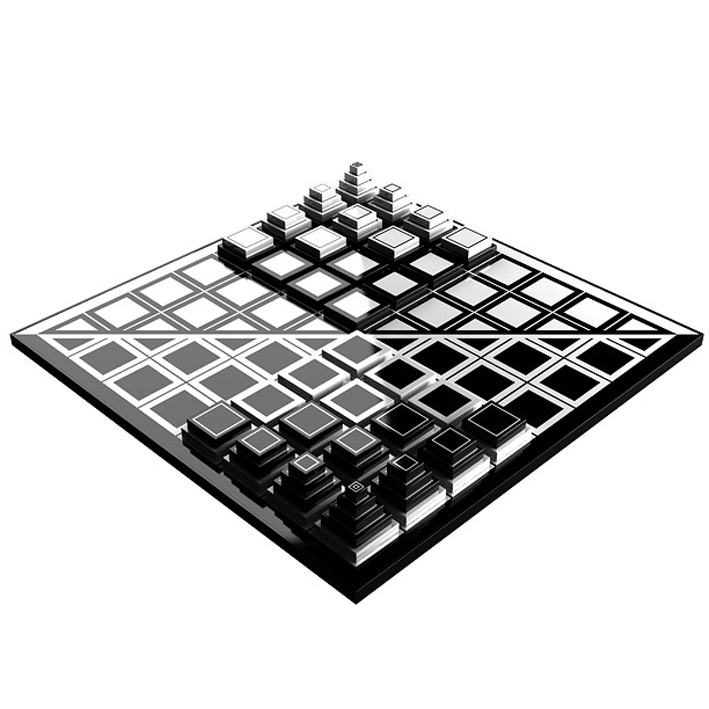
\includegraphics[scale=0.3]{img/game-cover.jpg}
\label{fig:0}
\end{center}
\end{figure}

Trench é um jogo de tabuleiro criado em Portugal por Rui Alípio Monteiro, em 2013.
O jogo de tabuleiro para 2 jogadores baseia-se na guerra de trincheiras da 1ª Guerra Mundial.

Os algoritmos aplicados no jogos seguem os princípios referidos no livro "The Art of the War", de Sun Tzu.

\subsection{Objetivos}

O objetivo do jogo é capturar todas as peças inimigas.
No entanto, nem sempre é possível que tal aconteça (pelas limitações das peças e do tabuleiro), pelo que a vitória ou a derrota regem-se por um sistema de pontuação, explicado em baixo.

\subsection{Modo de Jogo}

O jogador que possuir as peças de cor preta inicia o jogo.
Cada jogador tem direito a uma jogada por vez.
O jogo termina ao fim de 25 jogadas se nenhuma peça for capturada nesse intervalo.

\newpage

\subsection{Tabuleiro de Jogo}

O tabuleiro representa o campo de batalha, com as respetivas trincheiras.
Este tem uma forma em diamante (losango), dividido por uma linha diagonal, que representa a linha das trincheiras
(cada metade do tabuleiro tem uma cor predominante: preto para um jogador, branco para o outro).
O tabuleiro é constítuido por 64 casas (8x8), divididas em dois territórios opostos.

\begin{figure}[h!]
\begin{center}
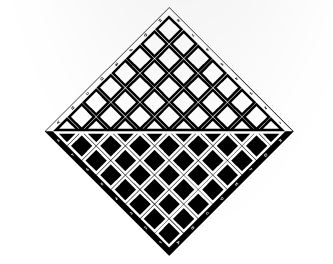
\includegraphics[scale=0.5]{img/board.jpg}
\caption{Tabuleiro de jogo 8x8}
\label{fig:1}
\end{center}
\end{figure}

\subsection{Peças do Jogo}

As peças do jogo são as apresentadas na seguinte tabela:

\begin{figure}[h!]
\begin{center}
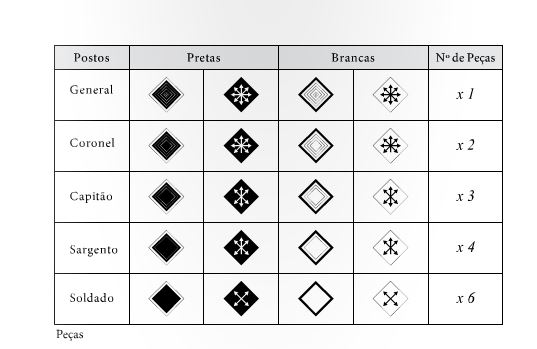
\includegraphics[scale=0.8]{img/pieces.jpg}
\caption{Tabel das peças do jogo}
\label{fig:2}
\end{center}
\end{figure}

\newpage

Estas possuem uma forma em losango, inspirada nas estrelas usadas pelos soldados em batalha e simbolizam a hierarquia militar em pirâmide.

\begin{figure}[h!]
\begin{center}

\includegraphics[scale=0.5]{img/piece.png}
\caption{Peça do jogo Trench}
\label{fig:3}
\end{center}
\end{figure}

As peças seguem a seguinte hierarquia (estando no topo o de mais alto nível):

\begin{enumerate}
  \item General
  \item Coronel
  \item Capitão
  \item Sargento
  \item Soldado
\end{enumerate}

\subsubsection{Disposição das Peças}
As peças são dispostas no tabuleiro de forma a simular a formação de um exército Romano, em diamante, como se poder ver na Fig. 5.
O general, a peça com maior ranking na hierarquia, fica no topo da metade aliada do tabuleiro, atrás de todo o exército.
Na linha da frente ficam os 6 soldados (possuem o menor ranking dentro da hierarquia).

\begin{figure}[h!]
\begin{center}
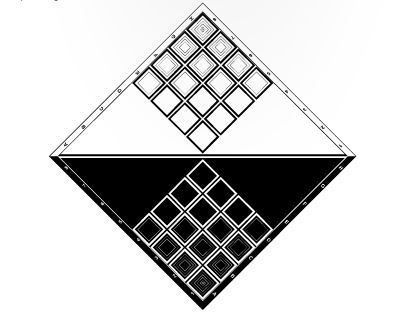
\includegraphics[scale=0.5]{img/pieces-disposition.jpg}
\caption{Disposição das peças do jogo}
\label{fig:4}
\end{center}
\end{figure}

\newpage

\subsubsection{Movimento das Peças}

\begin{itemize}
  \item \textbf{Soldado}: 1 casa (na diagonal em qualquer direção);
  \item \textbf{Sargento}: 2 casas (na diagonal em qualquer direção e para a frente);
  \item \textbf{Capitão}: 3 casas (na diagonal em qualquer direção e tanto para a frente como para trás);'
  \item \textbf{Coronel}: 4 casas (na diagonal em qualquer direção, para frente, esquerda e direita - mas não para trás);
  \item \textbf{General}: 5 casas (em todas as direções);
\end{itemize}

\begin{figure}[h!]
\begin{center}
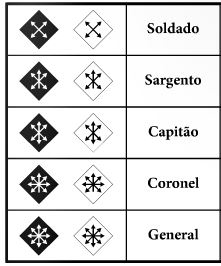
\includegraphics[scale=0.5]{img/pieces-movement.jpg}
\caption{Representação do movimento das peças do jogo}
\label{fig:5}
\end{center}
\end{figure}

\subsubsection{Restrições no Movimento das Peças}

\begin{itemize}
  \item O jogador é sempre obrigado a movimentar uma peça, na sua vez.
  \item Nenhuma das peças de jogo pode avançar sobre outra peça (seja do seu ou do exército adversário);
  \item Para capturar uma peça inimiga, a peça do jogador passa a ocupar a parcela quadrada da peça do adversário (terminando o movimento do jogador imediatamente).
  \item Nenhuma peça é obrigada a percorrer a totalidade das casas que pode percorrer. Isto é, por exemplo, o General pode-se mover apenas 1 casa ou 5 casas, conforme o jogador quiser.
\end{itemize}

\newpage

\subsection{A Trincheira}

A trincheira é representada pela linha horizontal no centro do tabuleiro, como referido anteriormente.
As peças nesta linha usufruem de um conjunto de vantagens e desvantagens:

\begin{itemize}
  \item \textbf{1ª Vantagem:} Uma peça na trincheira não pode ser atacada por uma peça adversária.
  \item \textbf{2ª Vantagem:} Uma peça na trincheira não é obrigada a parar quando ataca uma peça adversária. Portanto, essas podem continuar o seu movimento ou até atacar outras peças, até concluir a sua totalidade de casas a movimentar, ou o jogador decidir parar.

  \item \textbf{1ª Restrição:} Uma peça em trincheira não pode capturar peças adversárias que se encontrem no território aliado (retaguarda). Mas podem ser atacadas por peças adversárias que se encontrem no território aliado, sendo, aliás, a única forma para capturar peças inimigas na trincheira.
  \item \textbf{2ª Restrição:} O Coronel e o General podem-se movimentar ao longo de toda a linha da trincheira, mas não podem capturar nenhuma peça adversária que aí se encontre, ficando com os seus movimentos limitados.
\end{itemize}

\newpage

\subsection{Fim do Jogo}

O jogo termina ao fim de duas partidas. Depois de cada partida os jogadores trocam de lado, para que cada um jogue uma vez com as brancas e outra com as pretas.
  Uma partida termina quando algum jogador capturar todas as peças adversárias. No entanto, se após 50 jogadas ninguém capturar todas as peças adversárias o jogo termina e procede-se a contagem de pontos, segundo a seguinte tabela:

\begin{figure}[h!]
\begin{center}
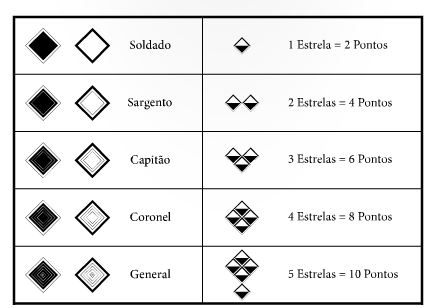
\includegraphics[scale=0.7]{img/points.jpg}
\caption{Valor de cada peça do jogo}
\label{fig:6}
\end{center}
\end{figure}

No final das duas partidas somam-se os pontos feitos por cada jogador em cada partida e ganha o jogo o jogador com mais pontos. Em caso de empate joga-se outra partida e ganha o jogo o jogador que conseguir capturar 40 pontos primeiro.

\newpage

%%%%%%%%%%%%%%%%%%%%%%%%%%
\section{Representação do Estado do Jogo}

A representação do estado do jogo irá ser feita através de uma lista de listas (matriz).
A matriz irá ser composta por uma lista contendo 15 listas de diferentes tamanhos, para se poder representar a forma em diamante do tabuleiro.
Portanto, a primeira e a última lista serão compostas por apenas 1 elemento, enquanto que a oitava lista, a do meio, correspondente à trincheira, será composta por 8 elementos.

Cada peça do jogo será representado pelo seguinte átomo:

\begin{itemize}
  \item{\textbf{Soldado:} So}
  \item {\textbf{Sargento:} Sa}
  \item{\textbf{Capitão:} Ca}
  \item{\textbf{Coronel:} Co}
  \item{\textbf{General:} G}
  \item{\textbf{Espaço Vazio:} E}
\end{itemize}

A cada uma destas peças (excepto as que representam o espaço vazio) será acrescentado um sufixo com o número do jogador.
Por exemplo, para o jogador 1, um soldado será representado por: 'So1'.

Para distinguir, no tabuleiro, a metade branca da metade preta, assume-se que a primeira
será sempre a metade superior do tabuleiro (logo, a metade do jogador 1),
sendo que a metade inferior será a preta (pertencente ao jogador 2).

Em Prolog a representação da matriz de jogo será a seguinte (vários casos):

\vspace{1cm}

\textbf{Estado inicial}

gameList( [ [g1],
    [co1, co1],
    [ca1, ca1, ca1],
    [sa1, sa1, sa1, sa1],
    [e, so1, so1, so1, e],
    [e, e, so1, so1, e, e],
    [e, e, e, so1, e, e, e],
    [e, e, e, so2, e, e, e],
    [e, e, so2, so2, e, e],
    [e, so2, so2, so2, e],
    [sa2, sa2, sa2, sa2],
    [ca2, ca2, ca2],
    [co2, co2],
     [g2]  ]).

\vspace{1cm}

\textbf{Estado final com todas as peças conquistadas (exemplo)}

gameList( [ [e],
    [co1, co1],
    [ca1, ca1, e],
    [sa1, e, sa1, sa1],
    [e, so1, e, so1, e],
    [e, e, so1, so1, e, e],
    [e, ca1, e, e, e, e, e],
    [e, e, e, e, g1, e, e],
    [e, e, sa1, e, e, e],
    [e, e, e, e, e],
    [e, e, e, so1],
    [e, e, e],
    [e, e],
     [e]  ]).

\vspace{1cm}

\textbf{Estado intermédio (exemplo)}

gameList( [ [e],
    [co1, co1],
    [ca1, ca1, e],
    [sa1, e, sa1, sa1],
    [e, so1, e, so1, e],
    [e, e, so1, so1, e, e],
    [e, ca1, e, e, e, e, e],
    [e, so2, e, e, g1, e, e],
    [e, e, sa1, e, e, e],
    [ca2, e, e, e, e],
    [e, e, e, so1],
    [e, g2, e],
    [e, e],
     [e]  ]).


\newpage

%%%%%%%%%%%%%%%%%%%%%%%%%%
\section{Visualização do Tabuleiro}

A representação do jogo na consola, em Prolog, está implementada da seguinte forma:

\begin{itemize}
  \item{\textbf{print\_board\_line:} imprime uma linha da matriz de jogo;}
  \item{\textbf{print\_board\_trench:} imprime a linha de trincheira (esta tem uma representção singular);}
  \item{\textbf{print\_board\_header:} imprime as duas coordenadas de topo;}
  \item{\textbf{print\_board\_footer:} imprime as duas coordenadas de fundo;}
\end{itemize}

\vspace{1cm}

\begin{lstlisting}
print_board([], _).

// print_board(GameList, LineIndex)
print_board([H|T], I) :-
                I \= 7, <-- trench line
                      I2 is I * 2,
                      S is abs(14 - I2),
                      print_spaces(S),
                      print_board_left_ref(I), <-- left rule
                      write('  '),
                      print_board_line(H),
                      write('  '),
                      print_board_right_ref(I), <-- right rule
                      nl,
                      I1 is I + 1,
                      print_board(T, I1);
                I2 is 7 * 2,
                      S is abs(14 - I2),
                      print_spaces(S),
                      write('   '),
                      print_board_trench(H),
                      nl,
                      I1 is 7 + 1,
                      print_board(T, I1).

// Prints the actual game line
print_board_line([]).

// Parameters: Game line to print (list)
print_board_line([H]) :-
                     get_board_symbol(H, S),
                     write(S).

print_board_line([H|T]) :-
                     get_board_symbol(H, S),
                     write(S),
                     write(' '),
                     print_board_line(T).

\end{lstlisting}

\newpage

\subsection{Visualização do Tabuleiro (continuação)}

\begin{lstlisting}

print_board_trench([]).

print_board_trench([H]) :-
                     get_board_symbol(H, S),
                     write(S).

print_board_trench([H|T]) :-
        get_board_symbol(H, S),
        write(S),
        format('~c', [215]), <-- caracter q simboliza a trincheira
        print_board_trench(T).

print_board_header(_) :-
        print_spaces(16),
        write('a'),
        print_spaces(3),
        write('i'), nl.

print_board_footer(_) :-
        print_spaces(16),
        write('p'),
        print_spaces(3),
        write('h'), nl.

\end{lstlisting}

\vspace{1cm}

\subsection{Visualização do Tabuleiro (output no Eclipse)}

\begin{figure}[h!]
\begin{center}
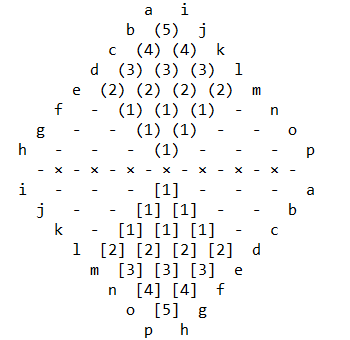
\includegraphics[scale=0.7]{img/output.png}
\caption{Output para a consola em Prolog}
\label{fig:7}
\end{center}
\end{figure}

\newpage

%%%%%%%%%%%%%%%%%%%%%%%%%%
\section{Movimentos}

\begin{lstlisting}

// movePiece(GameList, [From], [To], NewGameList).
move_piece(L, [X1, Y1], [X2, Y2], NL) :-
        convert_alpha_num(X1, R1),
        convert_alpha_num(Y1, C1),
        convert_alpha_num(X2, R2),
        convert_alpha_num(Y2, C2),
        get_piece(L, [R1, C1], P),
        can_move(L, [X1, Y1], [X2, Y2]), % Verifies if the move can be done
        set_piece(L, e, [R1, C1], L1),
        set_piece(L1, P, [R2, C2], NL).

// getPiece(GameList, [Row, Column], Piece).
//      Row and Columns must be in:         [1, 2, 3, 4, 5, 6, 7, 8]
get_piece(L, [R,C], P) :-
        convert_to_grid_pos(R, C, Row, Col),
        select_elem(Row, Col, L, P).


// setPiece(GameList, Piece, [Pos], NewGameList)
set_piece(L, P, [R, C], NL) :-
        convert_to_grid_pos(R, C, Row, Col),
        nth1(Row, L, X),
        replace(X, Col, P, Res),
        replace(L, Row, Res, NL).

// Predicate that checks if a given piece can move from a pos to another.
// canMove(GameList, [From], [To])
can_move(L, [R1, C1], [R2, C2]) :-
        get_piece(L, [R1, C1], PI),
        get_distance([R1, C1], [R2, C2], DIST),
        max_distance_for(PI, MAX),
        DIST < (MAX + 1),       <-- Distance verification
        get_direction(L, [R1, C1], [R2, C2], DIR),
        get_allowed_dir_for(PI, DIR).

\end{lstlisting}

\newpage

%%%%%%%%%%%%%%%%%%%%%%%%%%
\section{Computador (Inteligência Artificial)}

A inteligência artificial do jogo é realizada da seguinte forma: 



\begin{enumerate}

	\item Guardamos numa lista todas as jogadas possíveis para o computador (jogador 2)

	\item É escolhida dessa uma jogada, aleatoriamente. 

\end{enumerate}





\begin{lstlisting}



cpu_moves(GameList, Player, Moves) :-
        cpu_moves(GameList, Player, [1, 1], Moves).

cpu_moves(GameList, Player, [X, Y], Moves) :-
        Y == 9, Moves = [];

        X < 9,
                convert_alpha_num(R,X),
                convert_alpha_num(C,Y),
                get_piece(GameList, [R, C], P),
                check_piece_player(P, Player), !,
                cpu_piece_has_moves(GameList, [X, Y], [1, 1],
			 Player, PieceMoves), !,
                X1 is X + 1,
                cpu_moves(GameList, Player, [X1, Y], NewMoves),
                append([[R,C]],PieceMoves, NewPieceMoves),
                append([NewPieceMoves], NewMoves, Moves);
        
        X < 9, !,
                X1 is X + 1,
                cpu_moves(GameList, Player, [X1, Y], Moves);
        
        Y < 9, !,
                Y1 is Y + 1,
                cpu_moves(GameList, Player, [1, Y1], Moves).


\end{lstlisting}

\newpage

\begin{lstlisting}

cpu_piece_has_moves(GameList, [R,C], [TR,TC], 
			Player, PieceMoves) :-
        
        TC == 9, PieceMoves = [];
        
        TR < 9,
                NR is TR + 1,
                convert_alpha_point([A1,A2], [R,C]),
                convert_alpha_point([B1,B2], [TR,TC]),
                can_move(GameList, [A1, A2], 
			[B1, B2], Player), !,
                cpu_piece_has_moves(GameList, [R,C], 
			[NR,TC], Player, NewPieceMoves), !,
                append([[B1,B2]], NewPieceMoves, PieceMoves);
        
        TR < 9, !,
                NR is TR + 1,
                cpu_piece_has_moves(GameList, [R,C], [NR,TC],
			 Player, NewPieceMoves),
                append([], NewPieceMoves, PieceMoves);
        
        TC < 9, !,
                NC is TC + 1,
                cpu_piece_has_moves(GameList, [R,C], [1,NC],
			 Player, PieceMoves).


choose_cpu_move(_, Moves, [P1,P2], [T1,T2]) :-
        length(Moves, ML),
        random(1, ML, RandomRow),
        select_row(Moves, RandomRow, Row),
        select_col(Row, 1, [P1,P2]),
        length(Row, RL),
        random(2, RL, RandomCol),
        select_col(Row, RandomCol, [T1,T2]).



\end{lstlisting}

\newpage

%%%%%%%%%%%%%%%%%%%%%%%%%%
\section{Caso de fim do Jogo}

O jogo acaba nos seguintes cenários (não exatamente os do jogo original, mas apenas parte):

\begin{itemize}
  \item{\textbf{O jogador 1 já não tem peças em campo -} jogador 2 ganha;}
  \item {\textbf{O jogador 2 já não tem peças em campo -} jogador 1 ganha;}
  \item{\textbf{O jogador 1 já não tem movimentos válidos -} jogador 2 ganha;}
  \item{\textbf{O jogador 2 já não tem movimentos válidos -} jogador 1 ganha;}
\end{itemize}

\begin{lstlisting}

game_over(GameList) :-
        \+ player_has_pieces(GameList, p1),
                write('Player 1 has no pieces left.'), nl,
                write('Player 2 wins'), !, nl;
        \+ player_has_pieces(GameList, p2),
                write('Player 2 has no pieces left.'), nl,
                write('Player 1 wins'), !, nl;
        \+ player_has_moves(GameList, p1, 1, 1),
                write('Player 1 has no moves left.'), nl,
                write('Player 2 wins'), !, nl;
        \+ player_has_moves(GameList, p2, 1, 1),
                write('Player 2 has no moves left.'), nl,
                write('Player 1 wins'), !, nl.

// checks if the player has any piece remaining
player_has_pieces(GameList, Player) :-
        player_pieces(Player, L),
        player_has_pieces(GameList, L).

player_has_pieces([_|_], []) :- fail.

player_has_pieces(GameList, [P|R]) :-
        member_matrix(P,GameList);
        player_has_pieces(GameList, R).

\end{lstlisting}

\newpage

\subsection{Caso de fim do Jogo (continuação)}

\begin{lstlisting}

// checks if the player has any pieces width a valid move
player_has_moves(GameList, Player, X, Y) :-
        X < 9, Y < 9,
        get_piece(GameList, [X,Y], P),
        check_piece_player(P, Player),
        %write('> Piece: '), write(P), nl,
        piece_has_moves(GameList, [X,Y], [1,1]).

player_has_moves(GameList, Player, X, Y) :-
        %write('> FAILED'), nl,
        X < 9, !,
                X1 is X + 1,
                player_has_moves(GameList, Player, X1, Y);
        Y < 9, !,
                Y1 is Y + 1,
                player_has_moves(GameList, Player, 1, Y1);
        fail.

// checks if a piece has a valid movement to it
piece_has_moves(GameList, [X,Y], [A1,A2]) :-
        A1 < 9, A2 < 9,
        %get_piece(GameList, [X,Y], P),
        can_move(GameList, [X,Y], [A1,A2]).

piece_has_moves(GameList, [X,Y], [A1,A2]) :-
        A1 < 9, !,
                B1 is A1 + 1,
                piece_has_moves(GameList, [X,Y], [B1,A2]);
        A2 < 9, !,
                B2 is A2 + 1,
                piece_has_moves(GameList, [X,Y], [1,B2]);
        fail.

\end{lstlisting}

\newpage

%%%%%%%%%%%%%%%%%%%%%%%%%%
\section{Interface com o Utilizador}

A interacao com o utilizador é relativamente simples.

Para selecionar uma peça, o utilizador precisa de inserir duas coordenadas
(a interface fornece as coordenadas quando imprime o tabuleiro).

Para selecionar o destino da peca selecionada, o utilizador precisa de inserir as coordenadas de destino.

Obs.: A insercao de coordenadas é feita da seguinte forma: xy+ENTER, onde xy sao as duas coordenadas (em minuscula)
e ENTER a tecla homónima do teclado.

%\newpage
\vspace{1cm}

%%%%%%%%%%%%%%%%%%%%%%%%%%
\section{Conclusões}

Com a realização do primeiro trabalho prático proposto para a cadeira de PLOG conseguimos compreender e aplicar o paradigma da programação em lógica.  A forma de pensamento em Prolog é distinta daquilo a que estamos habituados pelo que a realização de um jogo de tabuleiro foi um grande desafio.



Consideramos que conseguimos implementar todas as funcionalidades base do jogo que nos foi proposto, no entanto a "inteligência artificial" necessitaria de um trabalho extra. Portanto, achamos que este seria o ponto que poderia ser trabalhado para tornar o projeto melhor, no sentido de tornar o computador mais inteligente na escolha das suas jogadas. 

\newpage

%%%%%%%%%%%%%%%%%%%%%%%%%%
\section{Bibliografia}

\vspace{1cm}

\begin{itemize}
  \item{\textbf{Replace method:} http://stackoverflow.com/questions/5850937/prolog-element-in-lists-replacement}
  \item{\textbf{List manipulation:} http://www.swi-prolog.org/pldoc/doc/swi/library/lists.pl}
  \item{\textbf{Moodle FEUP:} https://moodle.up.pt/course/view.php?id=2866}
\end{itemize}

%%%%%%%%%%%%%%%%%%%%%%%%%%
%%%%%%%%%%%%%%%%%%%%%%%%%%
\end{document}
